\documentclass{beamer}

\usepackage[utf8]{inputenc}
\usepackage[T1]{fontenc}
\usepackage[french]{babel}

\usepackage{lmodern}
\usepackage{csquotes}

\usepackage{graphics}

\usepackage{tikz}
\usetikzlibrary{arrows, positioning, fit, calc, arrows.meta} 
\tikzset{
    %Define standard arrow tip
    >=stealth',
    %Define style for boxes
    punkt/.style={
           rectangle,
           rounded corners,
           draw=black, very thick,
           text width=6.5em,
           minimum height=2em,
           text centered},
    % Define arrow style
    pil/.style={
           ->,
           thick,
           shorten <=2pt,
           shorten >=2pt,}
}

\tikzset{
  invisible/.style={opacity=0},
  visible on/.style={alt={#1{}{invisible}}},
  alt/.code args={<#1>#2#3}{%
    \alt<#1>{\pgfkeysalso{#2}}{\pgfkeysalso{#3}} % \pgfkeysalso doesn't change the path
  },
}

\usepackage{multirow}

\usetheme{metropolis}
 \metroset{block=fill}

\title{Imperfection et données géographiques}
\date{23 octobre 2018}
\author{Mattia Bunel}
\institute{Lastig--COGIT, IGN}


%\setbeamertemplate{frame footer}{Pied de page}

\begin{document}
  \maketitle

\begin{frame}{Plan du cours}
	  \setbeamertemplate{section in toc}[sections numbered]
	\tableofcontents%[hideallsubsections]
\end{frame}


\section*{Introduction}

\begin{frame}
  \begin{quote}
   \og À l’instar  d’autres  sciences,  la  Géographie  ne 
traite  pas  de  la  réalité  mais  de  modèles  de  la 
réalité \textelp{} \fg{}
\end{quote}
\hfill \href{https://hal.archives-ouvertes.fr/hal-01306283/}{Dutozia \emph{et al.} (2014)}
\end{frame}

\begin{frame}{Le problème de la représentation du réel}
	\begin{figure}
	\centering
	%
	\begin{tikzpicture}[auto]
	%
	% noeuds
	 %
 	\node [fill=black, text=white](incert) {Réalité};
	\node[below left= of incert, visible on = <2-> ] (impre) {Conceptualisation};
	\node[below right = of incert, visible on = <4->] (incom) {Implémentation};
	\node[below = of incert, visible on = <3->] (imp) {Modélisation};
	%
	% Liens
	%
	\draw[pil, ->,bend right=20, visible on = <2->](incert) to (impre);
	\draw[pil, ->, visible on = <3->](impre) to (imp);
	\draw[pil, ->, visible on = <4->](imp) to (incom);
	\end{tikzpicture}
	\end{figure}
\end{frame}

\section{Conceptualisation}
\subsection{Les imperfections du réel}

%%% Incertitudes
\begin{frame}{Incertitudes}
%
	\begin{figure}
		\centering
		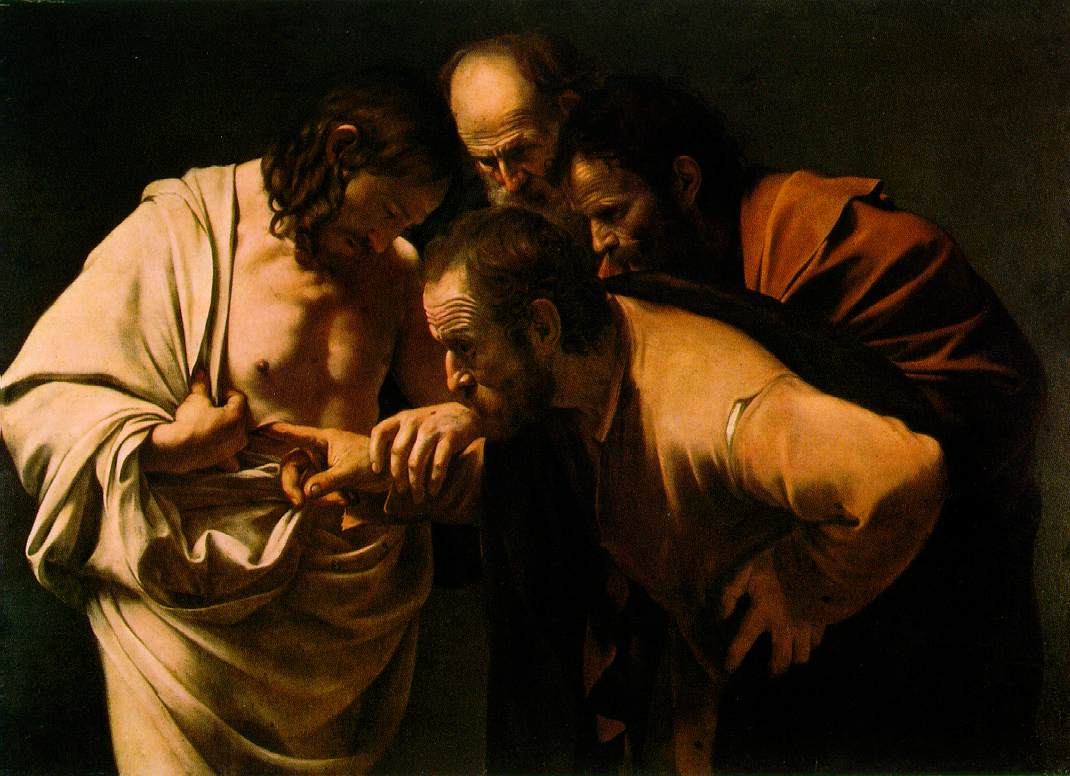
\includegraphics[height=0.6\textheight]{./Images/stthomas.png}
		%
		\caption{\emph{L'incrédulité de saint Thomas,} Le Caravage (1603)}
	\end{figure}
%
\alert{\emph{L'incertitude}} est  le doute sur la véracité d'une connaissance
\end{frame}

\begin{frame}{Incertitudes}
	\begin{figure}
		\centering
		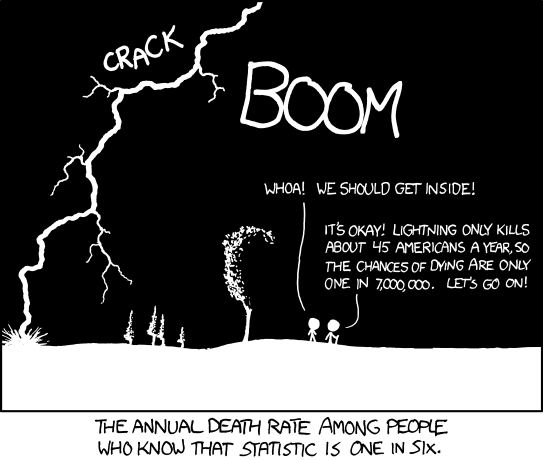
\includegraphics[height=0.59\textheight]{./Images/conditional_risk.png}
		%
		\caption{\href{https://www.xkcd.com/795/}{\emph{Conditional Risk,}} xkcd (2010)}
	\end{figure}
\alert{\emph{L'incertitude}} est \alert{contextuelle} et dépendante de l'observateur
\end{frame}

\begin{frame}{Incertitudes: exemple}
	\begin{figure}
		\centering
		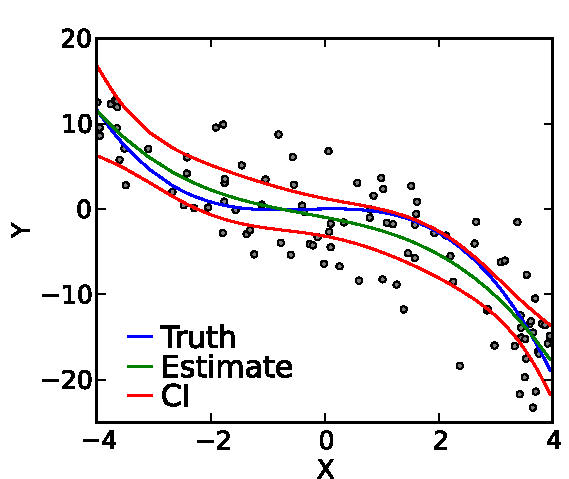
\includegraphics[height=0.6\textheight]{./Images/pg_scheffe.pdf}
		%
		\caption{\href{https://commons.wikimedia.org/wiki/File:Polyreg_scheffe.svg}{Régression polynomiale cubique avec intervalle de confiance,} Skbkekas (2009)}
	\end{figure}
\end{frame}

%%% Incomplétudes
\begin{frame}{Incomplétudes}
	\begin{figure}
		\centering
		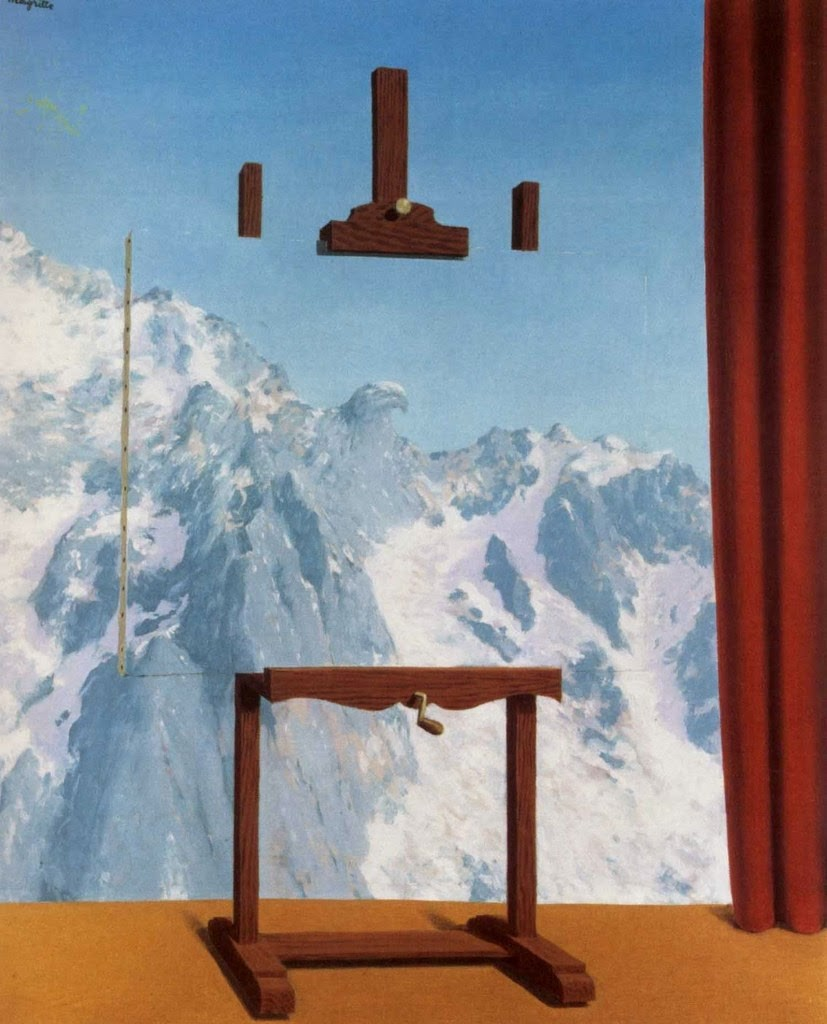
\includegraphics[height=0.59\textheight]{./Images/magritte.png}
		%
		\caption{\emph{L'appel des cimes,} René Magritte (1943)}
	\end{figure}
\alert{\emph{L'incomplétude}} désigne un manque de connaissances
\end{frame}

\begin{frame}{Incomplétudes: exemple (1)}
	\begin{table}
		\begin{tabular}{lcccc}
		\multicolumn{1}{l}{} & \multicolumn{4}{c}{Distributions} \\
			\cline{2-5}
                        & I & II & III & IV \\
			\hline
			\multicolumn{1}{l}{$\bar{x}$} & \multicolumn{4}{c}{9,0} \\
			\multicolumn{1}{l}{$\bar{y}$} & \multicolumn{4}{c}{7,5} \\
			\multicolumn{1}{l}{$V(x)$} & \multicolumn{4}{c}{10,0} \\
			\multicolumn{1}{l}{$V(y)$} & \multicolumn{4}{c}{3,75} \\
			\multicolumn{1}{l}{$\rho_{XY}$} & \multicolumn{4}{c}{0,816} \\
			\multicolumn{1}{l}{Éq. rég. lin.} & \multicolumn{4}{c}{$y=0.5x+3$} \\
			\hline
		 \end{tabular}
	\caption{Statistiques descriptives du quartet d'Anscombe}
	\end{table}
Les \alert{\emph{incomplétudes}} nécessitent des connaissances supplémentaires 
\end{frame}

\begin{frame}{Incomplétude: exemple (2)}
	\begin{figure}
		\centering
		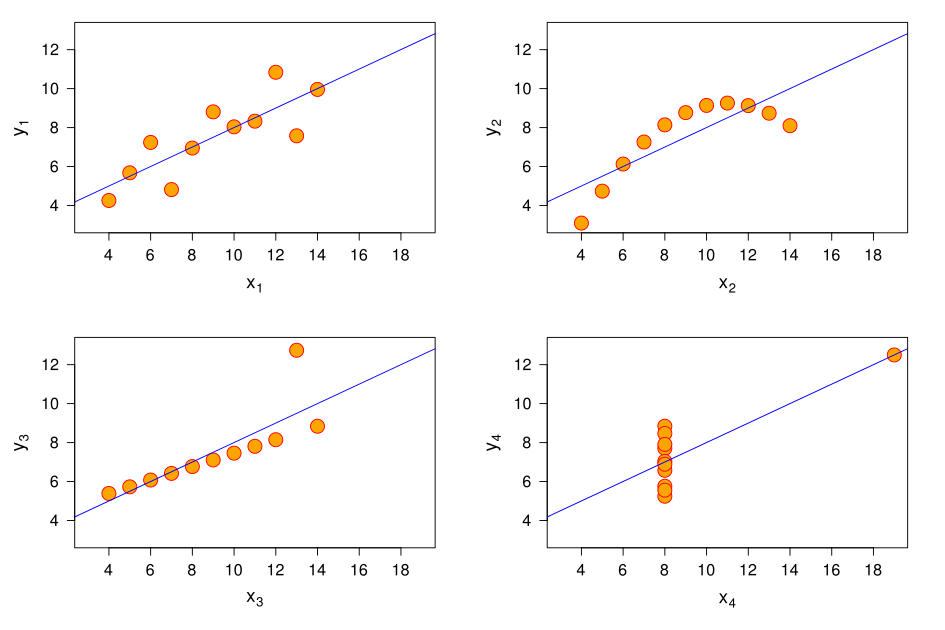
\includegraphics[height=0.59\textheight]{./Images/anscombe.png}
		%
		\caption{Représentation graphique du quartet d'Anscombe}
	\end{figure}
\end{frame}

%%% Imprécision
\begin{frame}{Imprécision}
	\begin{overprint}	
	\only<1,3>{
		\begin{figure}
			\centering
			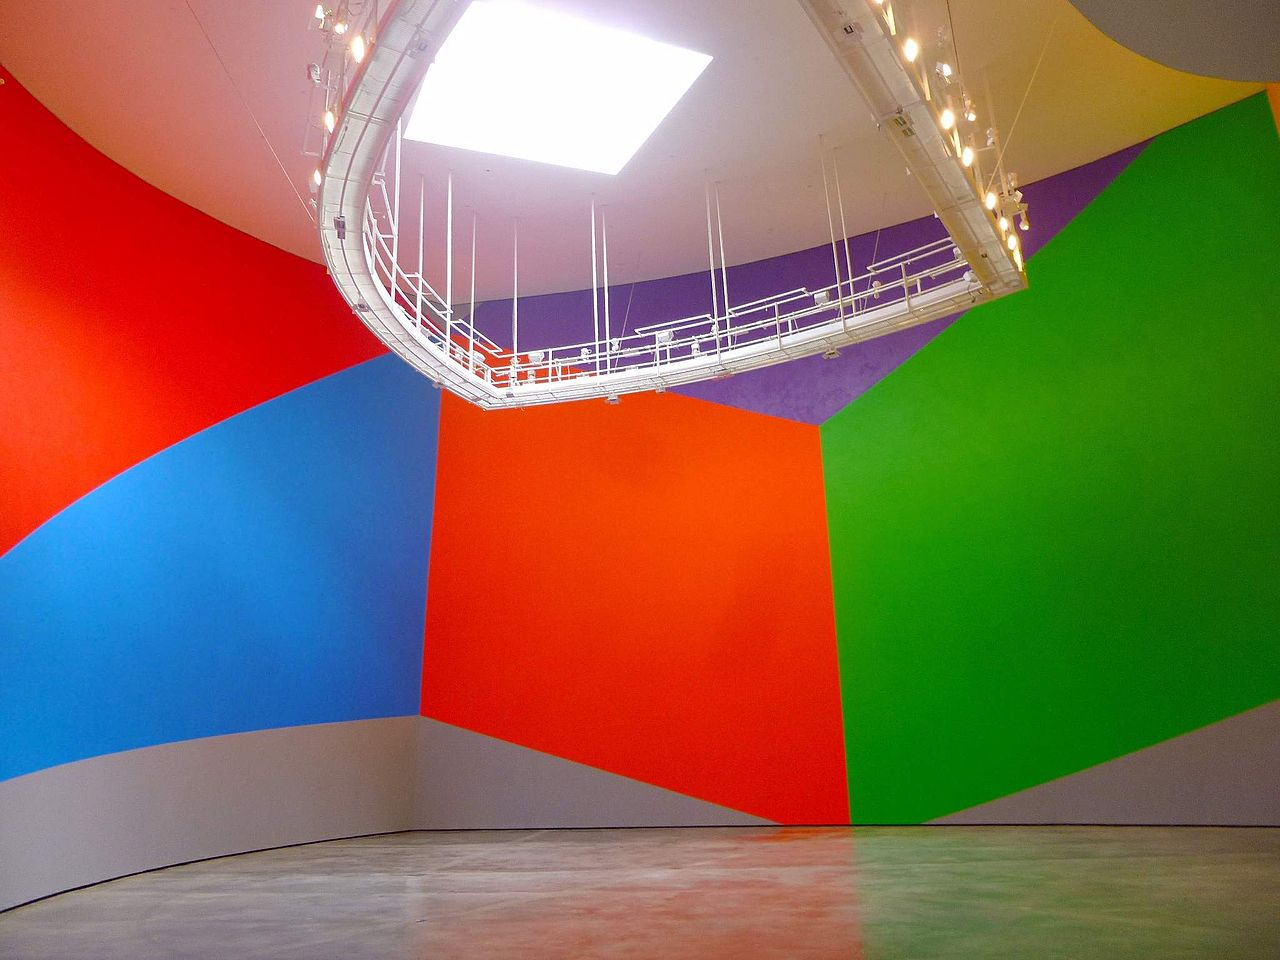
\includegraphics[height=0.59\textheight]{./Images/wd831.png}
			%
			\caption{\href{https://www.guggenheim-bilbao.eus/fr/oeuvres/murale-no831-formes-geometriques/}{\emph{Wall Drawing \#831,}} Sol LeWitt (1997)}
		\end{figure}
	}
	\only<2>{
		\begin{figure}
			\centering
			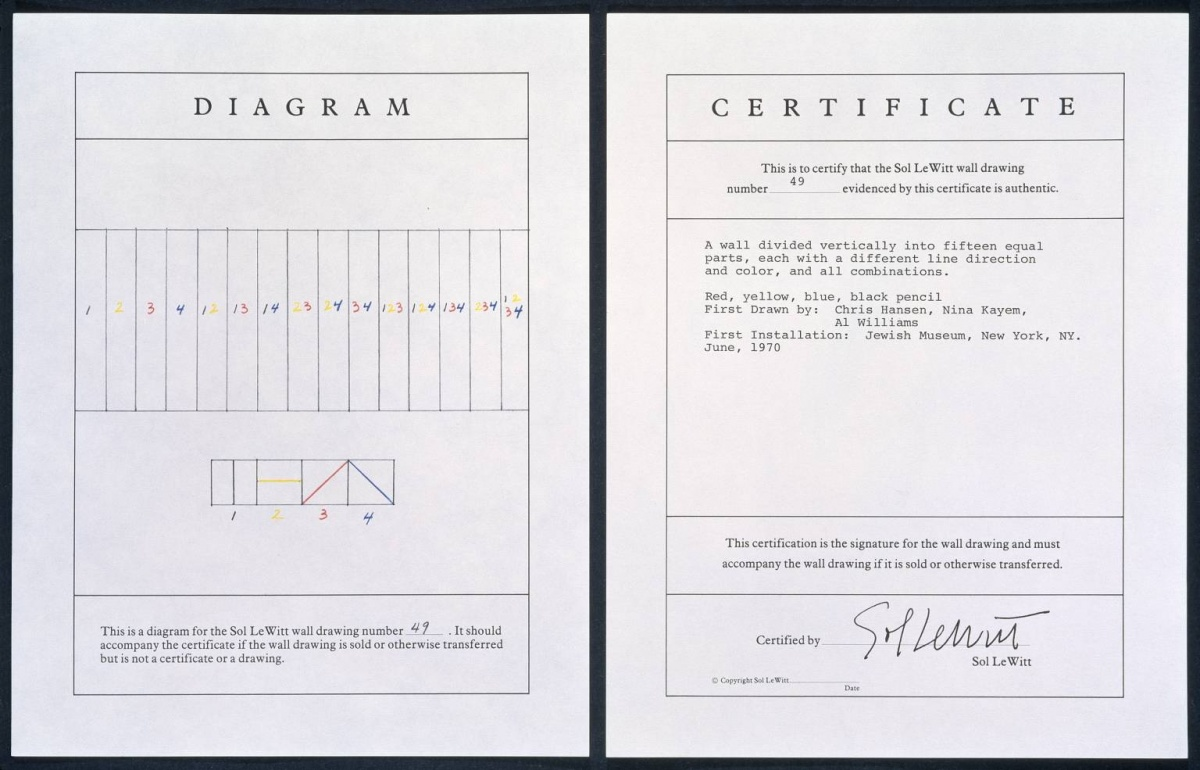
\includegraphics[height=0.59\textheight]{./Images/wd_certif.png}
			%
			\caption{\href{https://www.tate.org.uk/art/artworks/lewitt-a-wall-divided-vertically-into-fifteen-equal-parts-each-with-a-different-line-t01766}{Diagramme et certificat d’authenticité d'un \emph{Wall Drawing \#49,}} Sol LeWitt (1970)}
		\end{figure}
	}
	\alert{\emph{L'imprécision}} traduit une difficulté de délimitation 
	\end{overprint}
\end{frame}


\begin{frame}{Imprécision: exemple}
	\begin{figure}
		\centering
		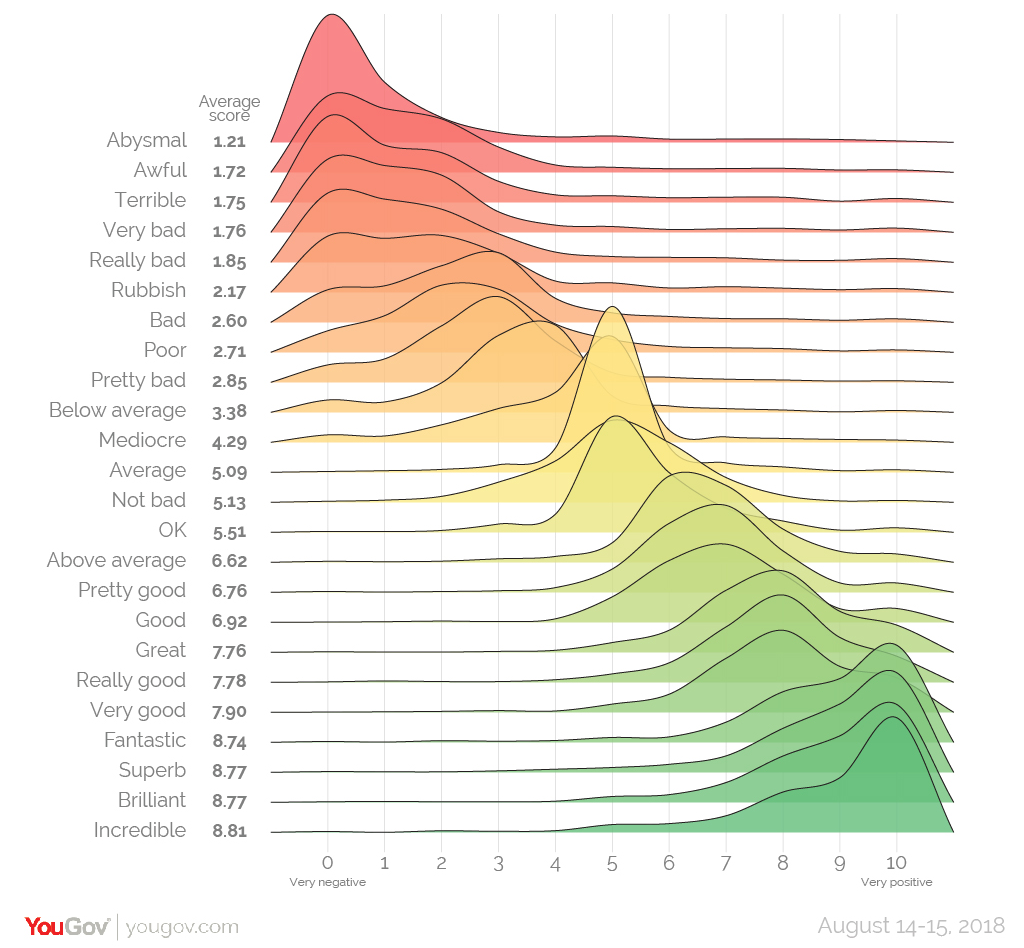
\includegraphics[height=0.59\textheight]{./Images/how_good_is_good.png}
		%
		\caption{\href{https://yougov.co.uk/news/2018/10/02/how-good-good/}{\emph{How Good is ''Good'',}} Matthew Smith (2018)}
	\end{figure}
\alert{\emph{L'imprécision}} est une caractéristique \alert{intrinsèque} de l'objet
\end{frame}

\begin{frame}{Pour résumer}
\alert{L'imperfection} regroupe :
	\begin{itemize}
		\item \alert{L'incertitude}
		\begin{itemize}
			\item Doute sur la véracité
			\item Contextuel
		\end{itemize}
		\item \alert{L'imprécision}
        \begin{itemize}
			\item Imprécisions numériques, catégories mal définies
			\item Propre à la connaissance 
		\end{itemize}
		\item \alert{L'incomplétude}
        \begin{itemize}
			\item Manque d'informations
			\item Contextuel
		\end{itemize}
	\end{itemize}
\end{frame}

%\begin{frame}{Pour résumer}
%Chaque type d'imperfection demande un \emph{traitement spécifique:}
%	\begin{itemize}
%		\item L'incertitude
%		\begin{itemize}
%			\item Théorie des probabilités
%			\item Théorie des possibilités
%		\end{itemize}
%		\item L'imprécision
%        \begin{itemize}
%			\item Théorie des sous-ensembles flous
%		\end{itemize}
%		\item L'incomplétude
%        \begin{itemize}
%			\item Théorie des fonctions de croyance
%		\end{itemize}
%	\end{itemize}
%\end{frame}

\begin{frame}{Des concepts liés}
	\begin{figure}
	\centering
	%
	\begin{tikzpicture}[node distance=1cm, auto]
	%
	% noeuds
	 %
 	\node[punkt] (incert) {Incertitude};
	\node[punkt, below right = of incert ] (impre) {Imprécision};
	\node[punkt, below left = of incert] (incom) {Incomplétude};
	%
	% Liens
	%
	\draw[pil, <-, bend right=20](incert) to (incom);
	%\draw[pil, <-, bend left=20](incert) to (impre);
	%\draw[pil, -, dashed](impre) to (incom);
	\end{tikzpicture}
	\caption{Liens entre concepts}
	\end{figure}
\end{frame}

 
 \begin{frame}{Des concepts liés}
	\begin{itemize}
		\item \alert{L'incomplétude} conduit à des \alert{incertitudes}\\
			\hspace{.25cm}{\small \emph{e.g.} je ne sais pas combien coûte une baguette, est-ce que j'ai assez d'argent sur moi ? }
	\end{itemize}
\end{frame}

\begin{frame}{Des concepts liés}
	\begin{figure}
	\centering
	%
	\begin{tikzpicture}[node distance=1cm, auto]
	%
	% noeuds
	 %
 	\node[punkt] (incert) {Incertitude};
	\node[punkt, below right = of incert ] (impre) {Imprécision};
	\node[punkt, below left = of incert] (incom) {Incomplétude};
	%
	% Liens
	%
	%\draw[pil, <-, bend right=20](incert) to (incom);
	\draw[pil, <-, bend left=20](incert) to (impre);
	%\draw[pil, -, dashed](impre) to (incom);
	\end{tikzpicture}
	\caption{Liens entre concepts}
	\end{figure}
\end{frame}

\begin{frame}{Des concepts liés}
\alert{L'imprécision} et \alert{l'incertitude} sont liées:
\begin{itemize}
	 \begin{overprint}
			\item Plus une assertion est précise, moins elle est certaine:\\
			\only<1,3>{\hspace{.25cm}{\small \emph{e.g.} je suis à environ 50 km \emph{vs} je suis à 55,32 km}\\}
		\only<2>{	
		\vspace{0.25cm}	
				{\small
				\emph{\og Dans toute statistique, l’inexactitude du nombre est compensée par la précision des décimales \fg{}}\\
				\hfill Alfred Sauvy}
			}			
		\only<3>{
			\item Un raisonnement basé sur des connaissances imprécises engendre des incertitudes:\\
				\hspace{.25cm}{\small \emph{e.g.} je roule \emph{vite,} suis-je en excès de vitesse ?}
		}
	\end{overprint}
\end{itemize}	
 \end{frame}
 
 \begin{frame}{Des concepts liés}
	\begin{figure}
	\centering
	%
	\begin{tikzpicture}[node distance=1cm, auto]
	%
	% noeuds
	 %
 	\node[punkt] (incert) {Incertitude};
	\node[punkt, below right = of incert ] (impre) {Imprécision};
	\node[punkt, below left = of incert] (incom) {Incomplétude};
	%
	% Liens
	%
	%\draw[pil, <-, bend right=20](incert) to (incom);
	%\draw[pil, <-, bend left=20](incert) to (impre);
	\draw[pil, -, dashed](impre) to (incom);
	\end{tikzpicture}
	\caption{Liens entre concepts}
	\end{figure}
\end{frame}

\begin{frame}{Des concepts liés}
	\begin{itemize}
		\item \alert{Isncomplétude} et \alert{imprécision} sont fréquemment associées \\
			\hspace{.25cm}{\small \emph{e.g.} modélisation à partir d'un échantillon}
	\end{itemize}
\end{frame}

\begin{frame}{Des concepts liés}
	\begin{figure}
	\centering
	%
	\begin{tikzpicture}[node distance=1cm, auto]
	%
	% noeuds
	 %
 	\node[punkt] (incert) {Incertitude};
	\node[punkt, below right = of incert ] (impre) {Imprécision};
	\node[punkt, below left = of incert] (incom) {Incomplétude};
	%
	% Liens
	%
	\draw[pil, <-, bend right=20](incert) to (incom);
	\draw[pil, <-, bend left=20](incert) to (impre);
	\draw[pil, -, dashed](impre) to (incom);
	\end{tikzpicture}
	\caption{Liens entre concepts}
	\end{figure}
\end{frame}


\subsection{Imperfections et objets spatiaux}

\begin{frame}{Comment étendre ces concepts aux objets spatiaux ?}
	\centering
	\begin{figure}
		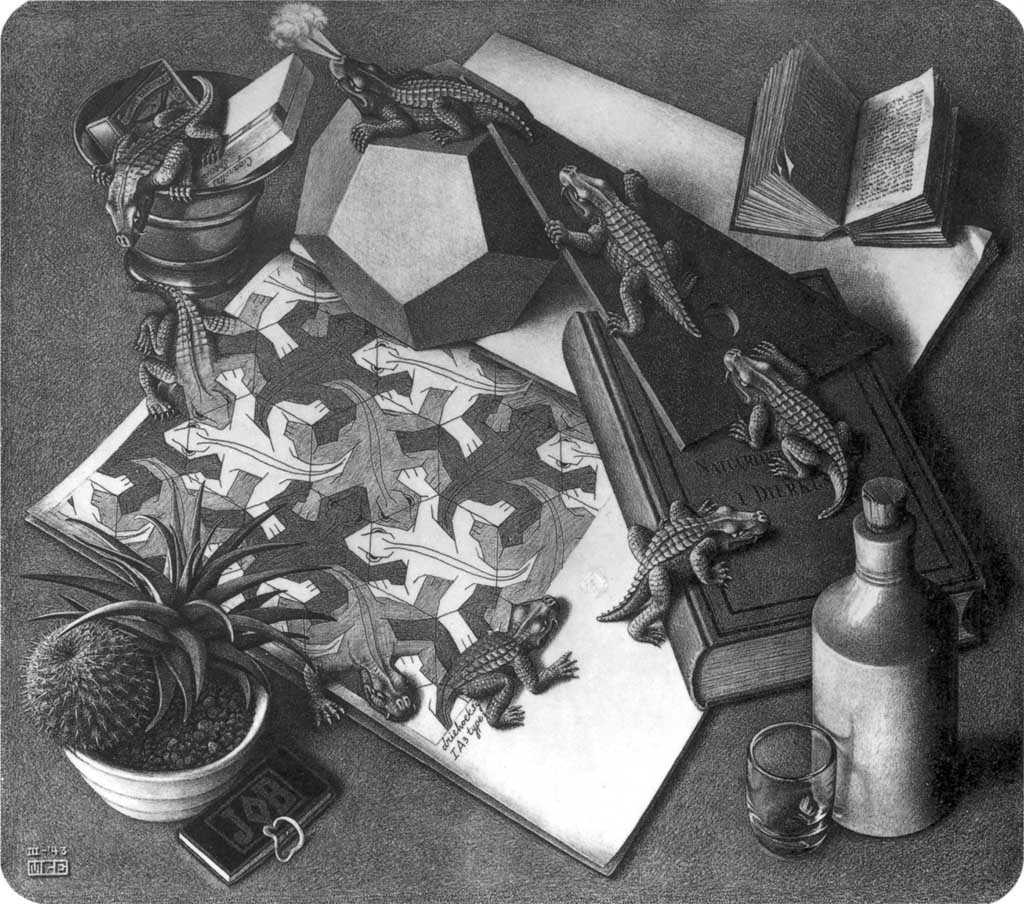
\includegraphics[height=0.6\textheight]{./Images/reptiles.png}
		%
		\caption{\href{https://en.wikipedia.org/wiki/Reptiles_(M._C._Escher)}{\emph{Reptiles,}} Maurits Cornelis Esher (1943)}
	\end{figure}
\end{frame}

\begin{frame}{Objets spatiaux}
	\begin{itemize}
		\item Le terme \alert{d'objet spatial} est ici utilisé dans le sens d'implémentation d'un \alert{objet géographique}
		\item Un \alert{objet spatial} est donc composé d'une \alert{géométrie} et des \alert{données attributaires} qui y sont potentiellement associées
		\item Ces deux composantes sont sujettes à des imperfections différentes, mais \alert{liées.}
		\item Nous ne parlerons ici que des \alert{imperfections géométriques}
	\end{itemize}
\end{frame}

\begin{frame}{Incomplétude et objets spatiaux}
Appliqué à la géométrie le concept d'incomplétude caractérise des géométries dont certaines parties sont manquantes
{\small \emph{e.g.} géométrie non terminées}

 \begin{alertblock}{Attention}
	Ne pas confondre avec l'incomplétude de la base de données (\emph{e.g.} petits bâtiments non tracés)
 \end{alertblock}

\end{frame}

\begin{frame}{Incertitude et objets spatiaux}
Appliquée à la géométrie l'incertitude est le doute sur la véracité de celle-ci.

On peut distinguer deux formes d'incertitude géométrique:
	\begin{itemize}
		\item \alert{Incertitude positionnelle} \\
			\hspace{.25cm}{\small \emph{i.e.} Le doute sur la position d'un objet spatial}
		\item \alert{Incertitude morphologique} \\
			\hspace{.25cm}{\small \emph{i.e.} Le doute sur la forme d'un objet spatial}
	\end{itemize}  
\end{frame}

\begin{frame}{Incertitude positionnelle}
\begin{figure}
		\centering
		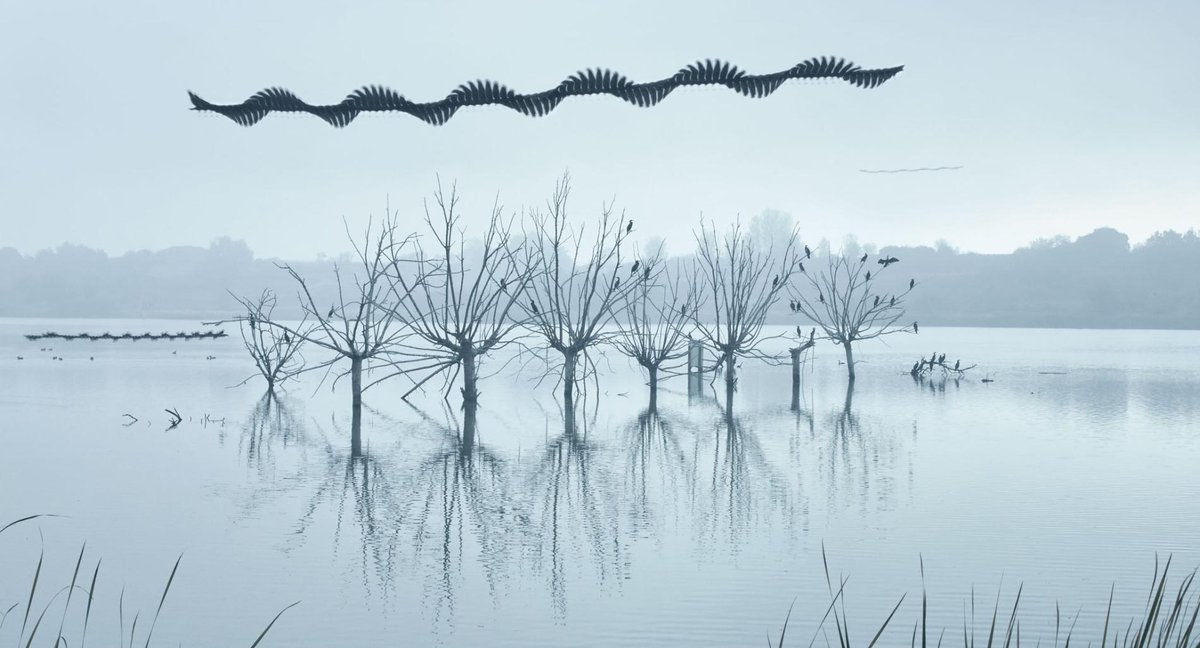
\includegraphics[height=0.59\textheight]{./Images/birds.png}
		%
		\caption{\href{https://www.nationalgeographic.com/magazine/2018/01/photo-journal-birds-paths-migration-starling/}{\emph{If Birds Left Tracks in the Sky, They’d Look Like This,}} National Geographic (2018)}
	\end{figure}
\end{frame}

\begin{frame}{Incertitude morphologique}
	\begin{figure}
		\centering
		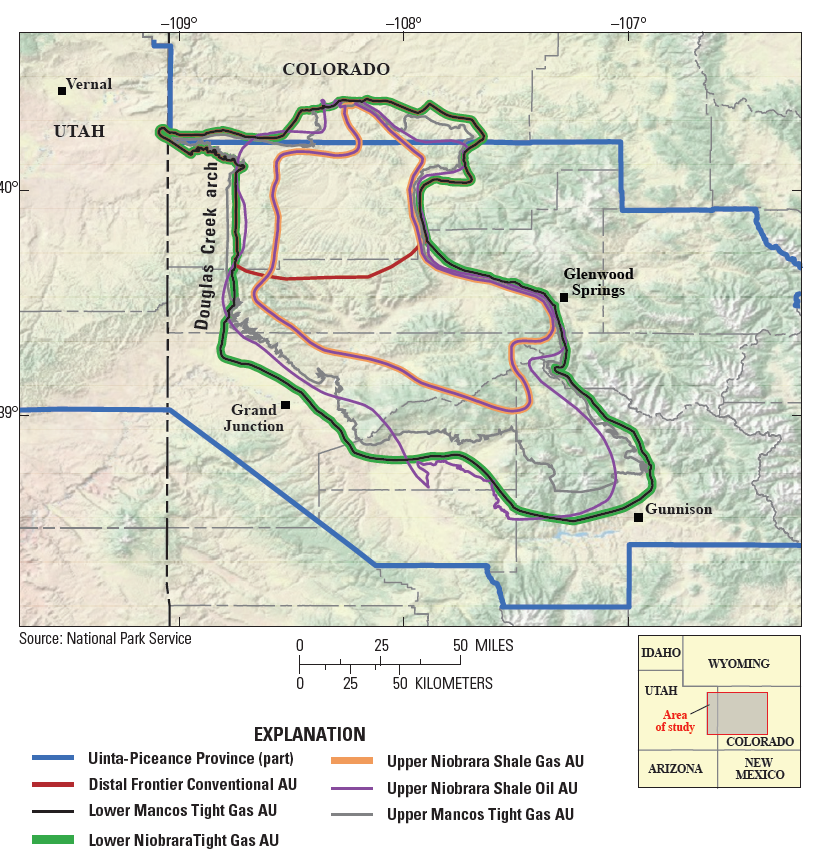
\includegraphics[height=0.59\textheight]{./Images/mancos.png}
		%
		\caption{\href{https://www.usgs.gov/media/images/2016-mancos-assessment-map}{\emph{Mancos Assessment Map,}} USGS (2016)}
	\end{figure}
\end{frame}

\begin{frame}{Imprécision et objets spatiaux}
\alert{L'imprécision géométrique} est la difficulté à fixer des limites nettes aux objets spatiaux.

{\small \emph{e.g.} limites d'une ville, d'une forêt, d'une mer, etc.}

 \begin{alertblock}{Attention}
  	C'est une notion \textbf{très} différente de \emph{l'incertitude morphologique}. \small {un objet 
  	spatial imprécis est de forme et de position connue.}
 \end{alertblock}
\end{frame}

\begin{frame}{Imprécision spatiale}
\begin{figure}
		\centering
		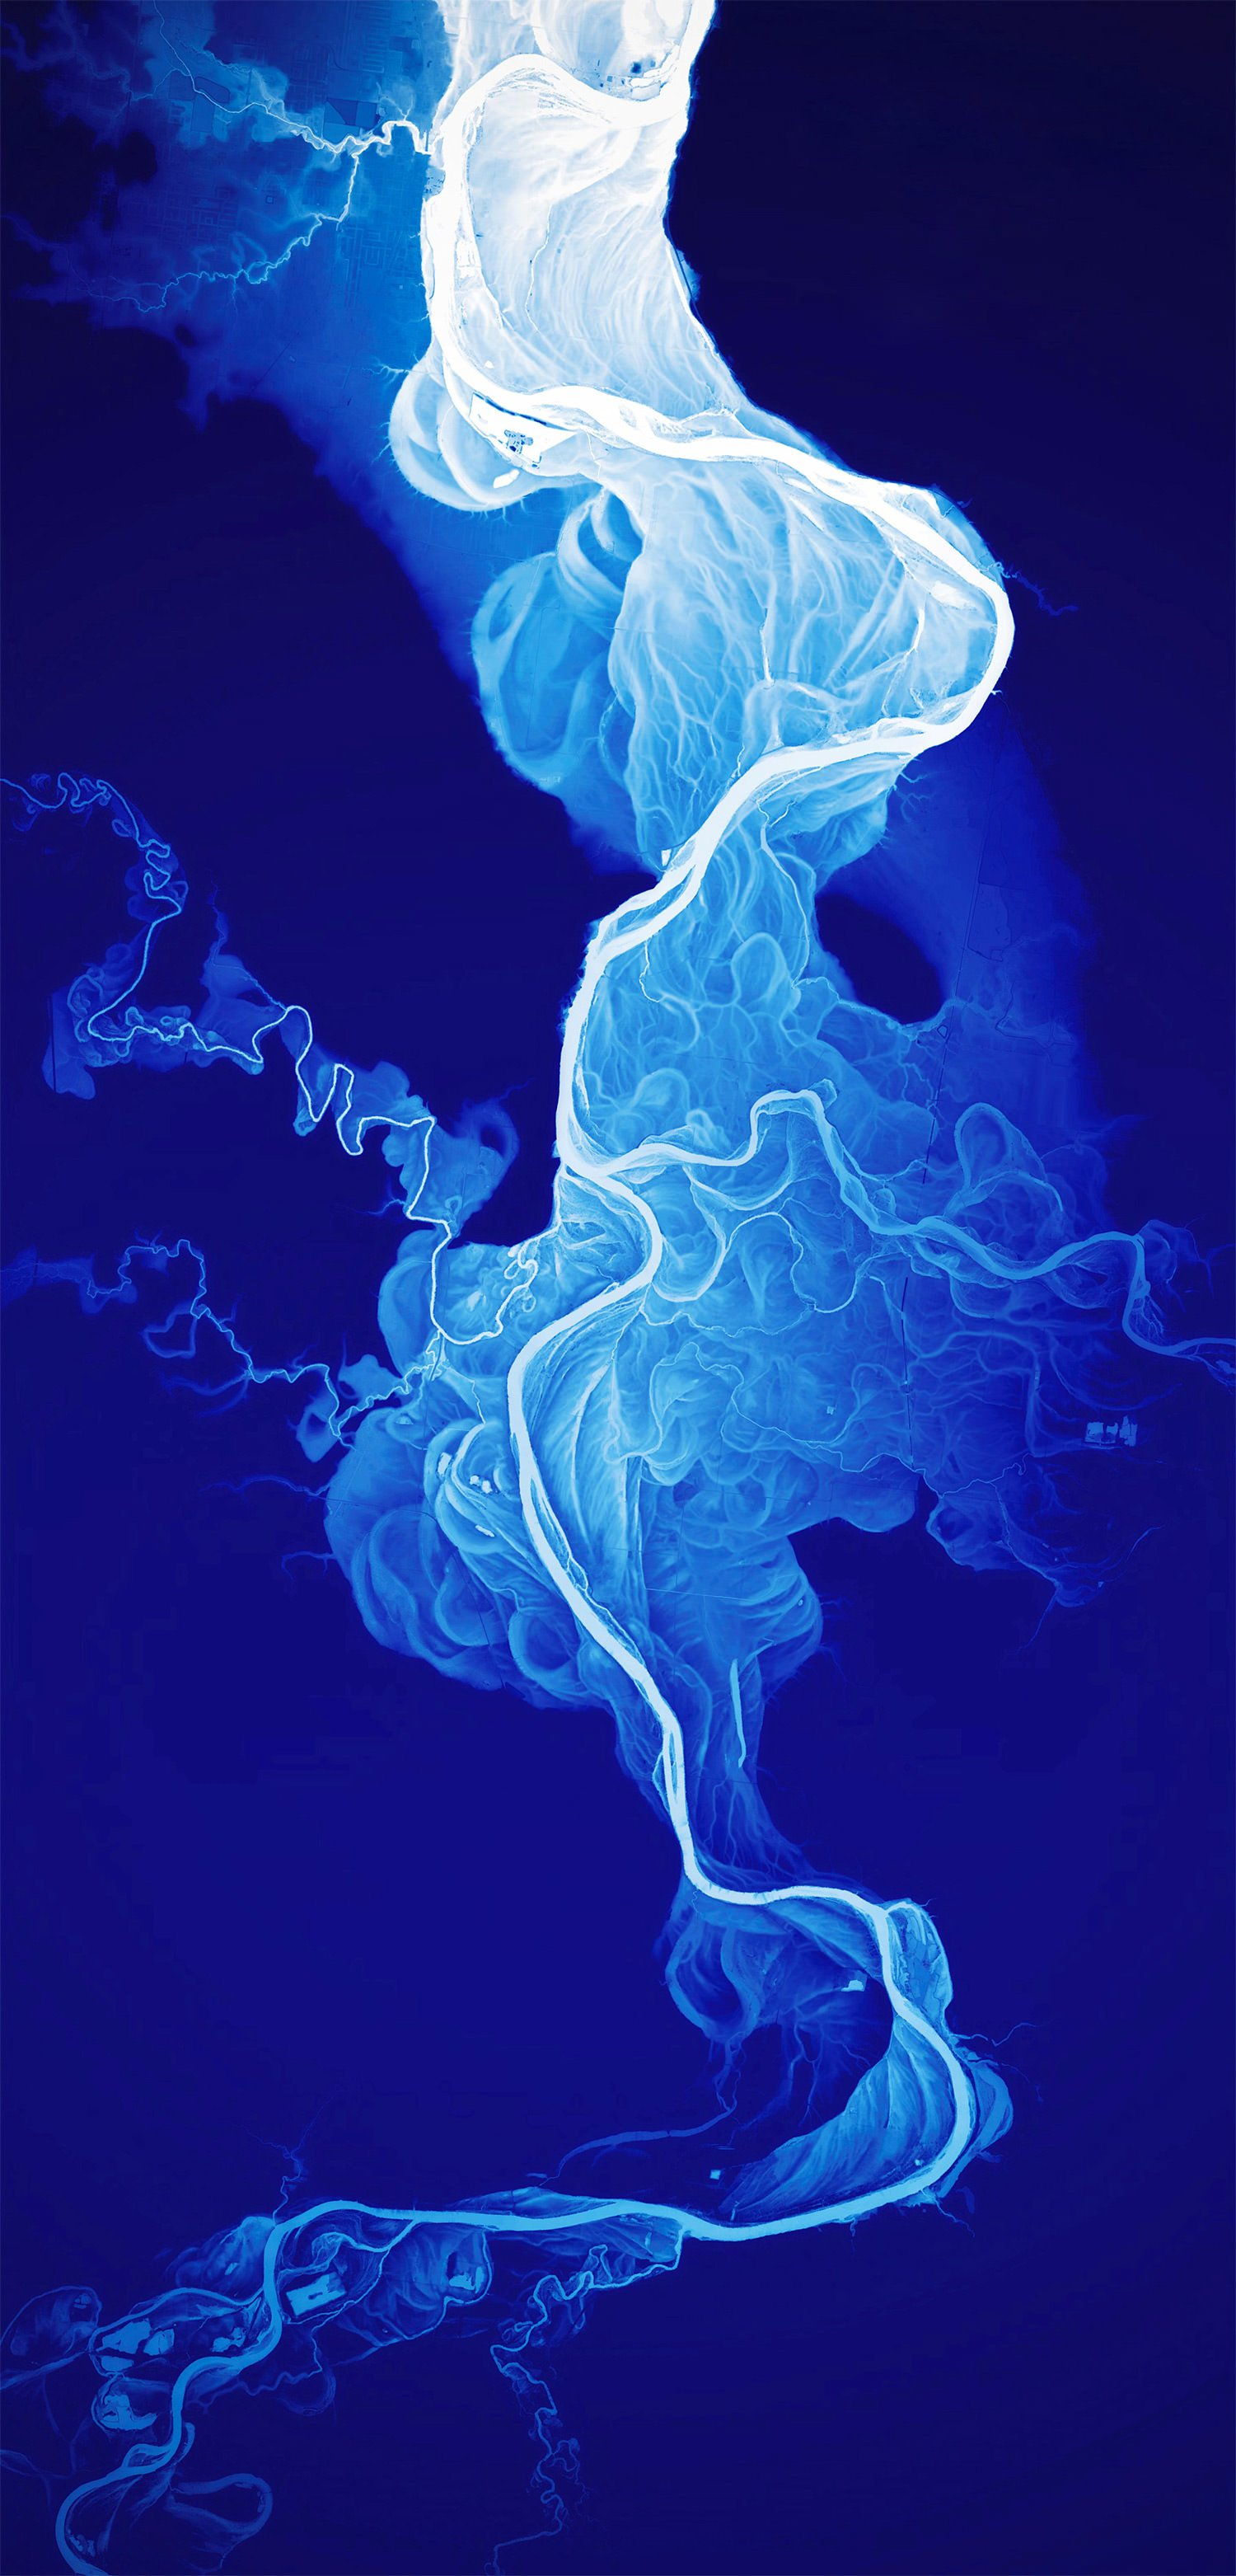
\includegraphics[angle=90, height=0.59\textheight]{./Images/river.png}
		%
		\caption{\href{https://www.oregongeology.org/pubs/ll/p-poster-willamette.htm}{\emph{Willamette River Historical Stream Channels, Oregon,}} Daniel E. Coe (2006)}
	\end{figure}
\end{frame}

\begin{frame}{Imprécision spatiale}
	\begin{figure}
		\centering
		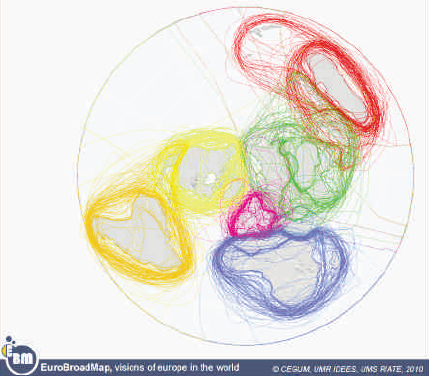
\includegraphics[height=0.6\textheight]{./Images/didelon.png}
		%
		\caption{\href{https://www.researchgate.net/publication/322860813_UN_MONDE_D'INTERSTICES_Apport_de_la_logique_floue_pour_l'analyse_des_cartes_interpretatives}{\emph{Un monde d'interstices,}} Didelon \emph{et al.} (2011)}
	\end{figure}
\end{frame}

\begin{frame}{Incertitude \emph{vs} imprécision}
		\begin{figure}
		\centering
		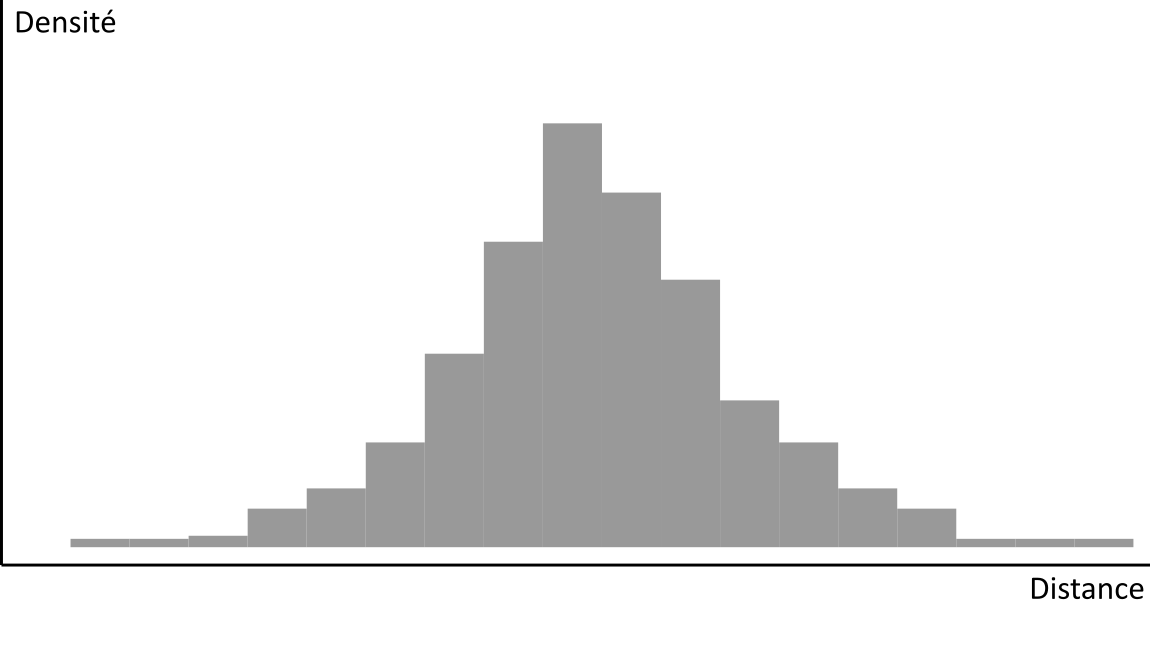
\includegraphics[height=0.6\textheight]{./Images/imp_incert_1.png}
		%
		\caption{Distribution de densités}
		\end{figure}
\end{frame}

\begin{frame}{Incertitude \emph{vs} imprécision}
		\begin{figure}
		\centering
		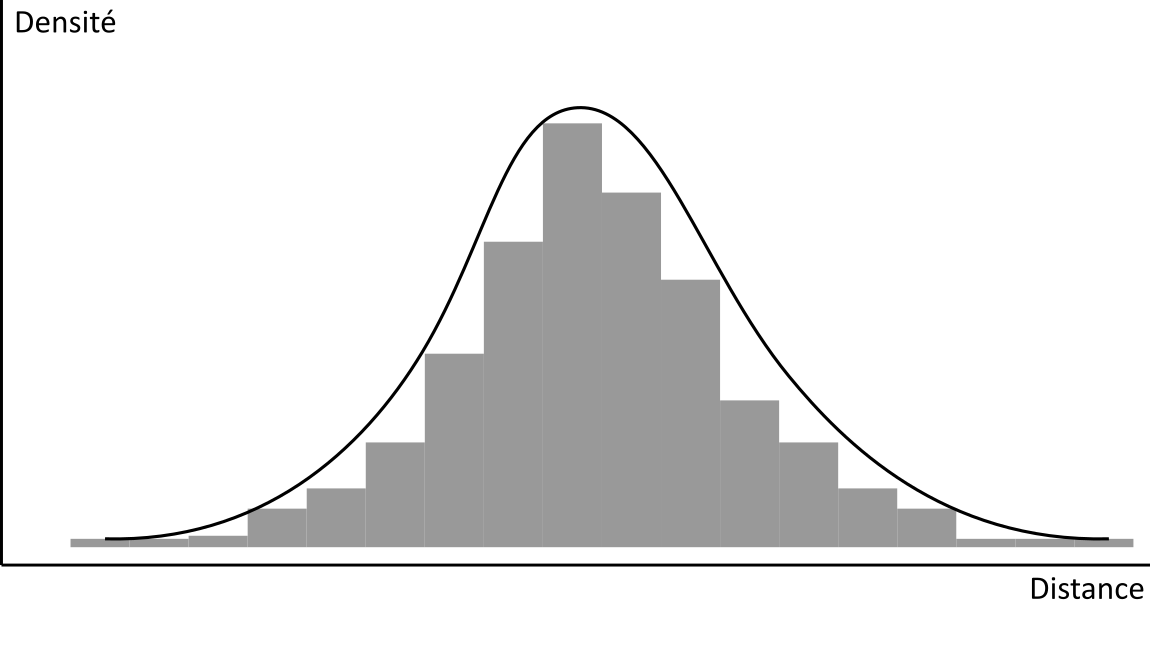
\includegraphics[height=0.6\textheight]{./Images/imp_incert_2.png}
		%
		\caption{Génération du modèle}
		\end{figure}
\end{frame}

\begin{frame}{Incertitude \emph{vs} imprécision}
		\begin{figure}
		\centering
		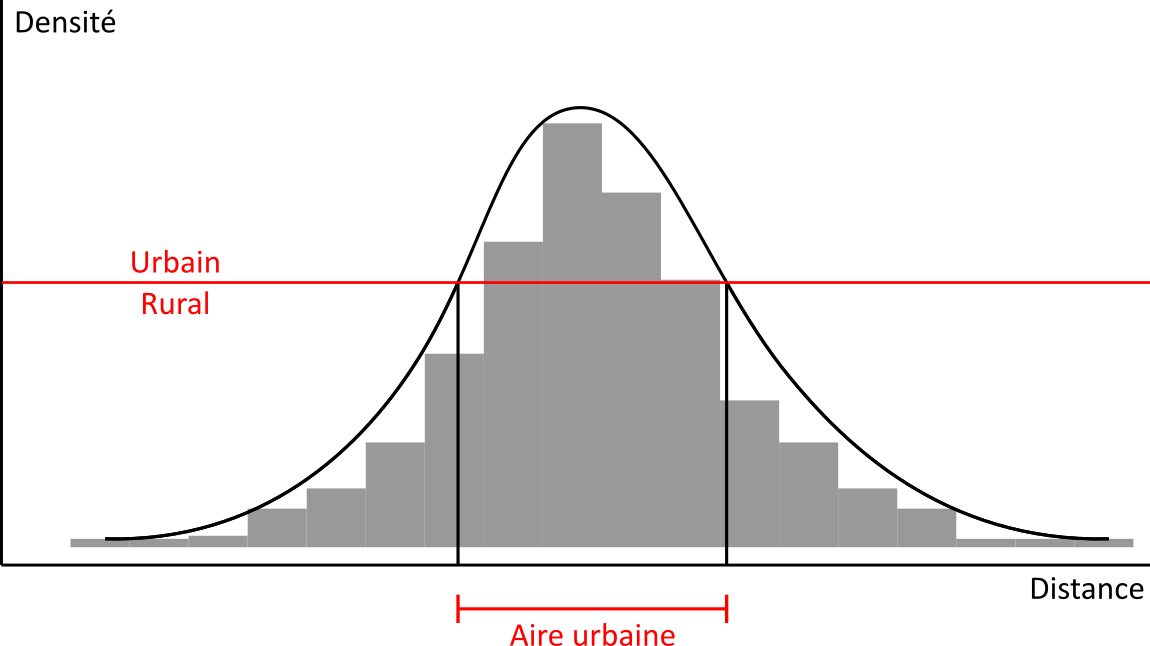
\includegraphics[height=0.6\textheight]{./Images/imp_incert_3.png}
		%
		\caption{Délimitation urbain / rural}
		\end{figure}
\end{frame}


\begin{frame}{Incertitude \emph{vs} imprécision}
		\begin{figure}
		\centering
		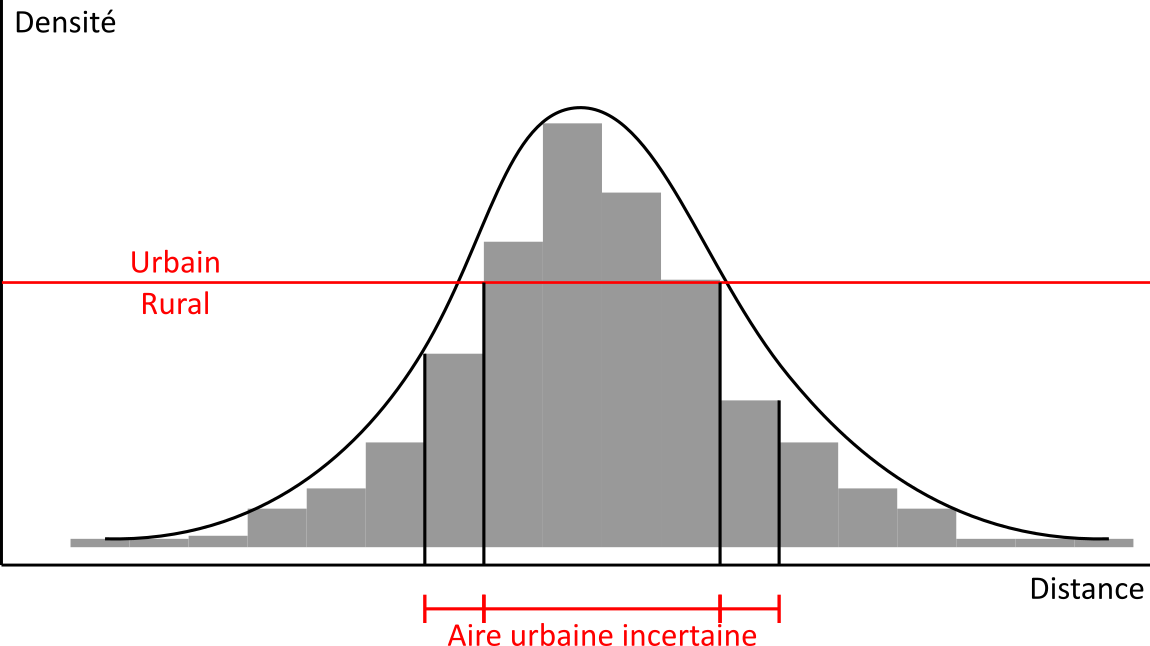
\includegraphics[height=0.6\textheight]{./Images/imp_incert_4.png}
		%
		\caption{Délimitation incertaine}
		\end{figure}
\end{frame}



\begin{frame}{Incertitude \emph{vs} imprécision}
		\begin{figure}
		\centering
		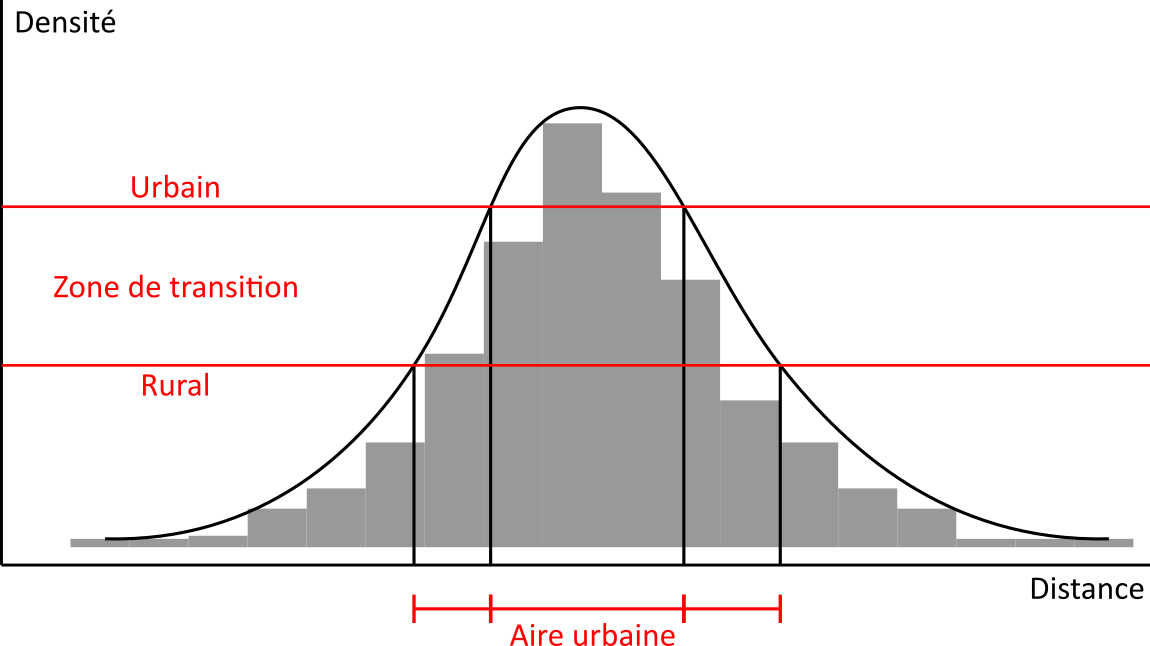
\includegraphics[height=0.6\textheight]{./Images/imp_incert_5.png}
		%
		\caption{Délimitation floue}
		\end{figure}
\end{frame}


\begin{frame}{Pour résumer}
	\begin{figure}
		\begin{tikzpicture}[scale=0.45, on grid]
			\newcommand{\yslant}{0.5}
			\newcommand{\xslant}{-0.75}
			\tikzstyle{level 1}=[level distance=3.5cm, sibling distance=3.5cm]
			%
			\begin{scope}[yshift=-150,yslant=\yslant,xslant=\xslant,		
					every node/.append style={yslant=\yslant,xslant=\xslant}]
					%
					\node (i) {\tiny Imperfection}
						child {node (imp) {\tiny Imprécision}}
						child {node (inco) {\tiny Incomplétude}}
						child {node(inc) {\tiny Incertitude}};
					%
					\draw node [black, 
						thin, draw, rectangle, fill=black, fill opacity=0.1,
						fit={(-.75,3) (0.75,-7)}] (rec){}; 
			\end{scope}
			%
			\begin{scope}[yshift=0,yslant=\yslant,xslant=\xslant,		
				every node/.append style={yslant=\yslant,xslant=\xslant}]	
				%
					\node (obj) {\tiny Objet spatial} 			
						child {node(geom) {\tiny Géométrie}}
						child {node(att) {\tiny Attributs}};
						%
					\draw node [black, 
						thin, draw, rectangle, fill=black, fill opacity=0.1,
						fit={(-.75,3) (0.75,-7)}] (rec2){}; 
			\end{scope}
			%
		 	\draw [->,  red, visible on = <2-5>] (inc.north) to (geom.south);
		 	\draw [->,  red, visible on = <3-5>] (inc.north) to (att.south);
		 	\fill[red, fill opacity=.1, visible on = <4>] (inc.north) -- (geom.south) -- (att.south) -- cycle;
		 	\draw [->,  red, visible on = <5>] (inc.north) to (obj.south) ;
		 	%%
		  	\draw [->,  red, visible on = <6-8>] (imp.north) to (geom.south);
		 	\draw [->,  red, visible on = <7-8>] (imp.north) to (att.south);
		 	\fill[red, fill opacity=.1, visible on = <8>] (imp.north) -- (geom.south) -- (att.south) -- cycle;
		 	%%
		  	\draw [->,  red, visible on = <9->] (inco.north) to (geom.south);
		 	\draw [->,  red, visible on = <10->] (inco.north) to (att.south);
		 	\fill[red, fill opacity=.1, visible on = <11>] (inco.north) -- (geom.south) -- (att.south) -- cycle;
			%
			\draw [dotted] (rec.north east) -- (rec2.north east);
		 	\draw [dotted] (rec.south east) -- (rec2.south east);
		  	\draw [dotted] (rec.south west) -- (rec2.south west);	
		  	\draw [dotted] (rec.north west) -- (rec2.north west);
		\end{tikzpicture} 
	\caption{Imperfection et objets spatiaux}
	\end{figure}
\end{frame}

\begin{frame}{Pour résumer}
	\begin{itemize}
		\item \alert{L'imprécision, l'incertitude et l'incomplétude} concernent les objets spatiaux
		\item Il faut distinguer \alert{l'imperfection de la géométrie} et celle des \alert{attributs} (même si un lien peut exister)
		\item Il faut distinguer \alert{l'imperfection d'un objet spatial} de celle d'une \alert{classe d'objets}  
	\end{itemize}
\end{frame}


\section{Modèles théoriques}
\subsection{Modèles exacts}

\begin{frame}{Modèles \og exacts \fg}
		Les modèles dit \og exacts \fg proposent de modéliser des géométries imprécises à l'aide d'une extension du modèle \emph{simple features}
	
	C'est une voie particulièrement bien explorée, de nombreux modèles ont étés proposés:
	\begin{itemize}
		\item Le modèle \emph{egg-yolk,} Cohn et Gotts (1996)
		\item Les propositions de Clementini et Di Felice (1996, 2005, 2008)
		\item Le modèle de Schneider basé sur l’approche Realm/ROSE (1996)
		\item Le modèle d’Erwig et Schneider (1997)
		\item Le modèle de Bejaoui (2009)
	\end{itemize}
\end{frame}

\begin{frame}{le modèle \emph{egg-yolk} (1996)}
	\begin{overprint}
		\only<1,3>{
			 \begin{alertblock}{Proposition}
			 	\begin{itemize}
			 		\item Étendre les régions du modèle \emph{simple features}
			 		\item Modéliser des régions avec deux frontières
				\end{itemize}  
			\end{alertblock}
		}
		\only<3>{
			\begin{exampleblock}{Limites}
				 \begin{itemize}
			 		\item Ne permet que la modélisation de régions
			 		\item Appartenance discrète
				\end{itemize}  
			\end{exampleblock}
		}
		\only<2>{
			\begin{figure}
				\centering
				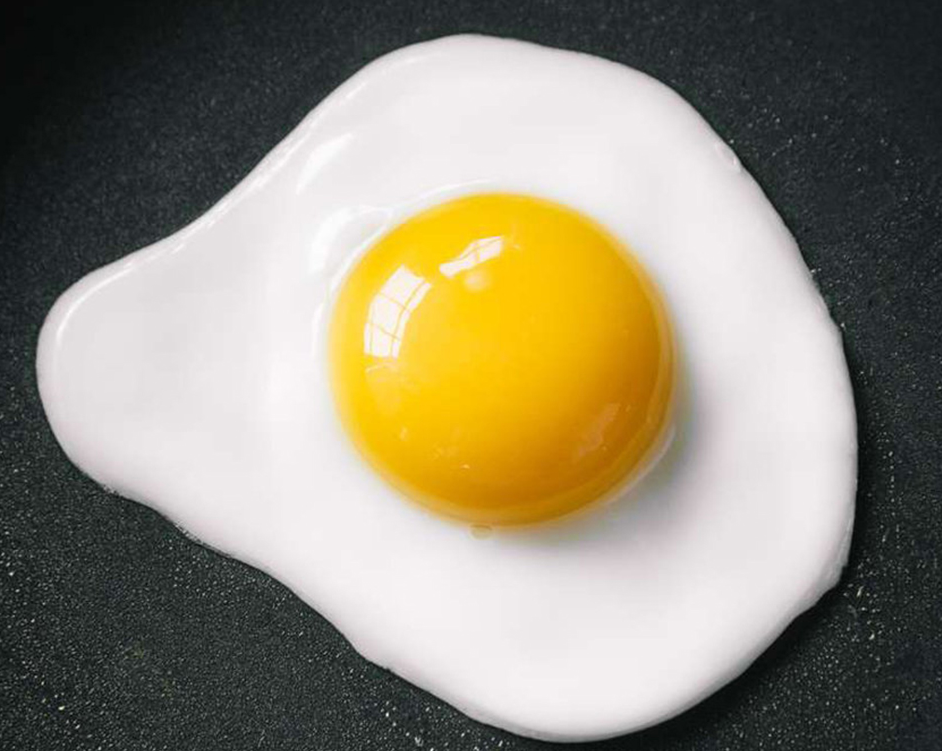
\includegraphics[height=0.7\textheight]{./Images/yolk.png}
				%
				\caption{Un œuf au plat}
			\end{figure}
		}
	\end{overprint}	
\end{frame}

\begin{frame}{Les travaux de Clementini et Di Felice}
	\begin{overprint}
		\only<1,3>{
			\begin{alertblock}{Proposition}
				\begin{itemize}
					\item Modéliser des régions avec deux frontières
					\item Modélisation des points sous la forme d'une région représentant l'ensemble des positions possibles
					\item Modélisation des lignes à l'aide de points vagues (début et fin) et d'un ensemble de lignes (chemins possibles)
				\end{itemize}  
			\end{alertblock}
		}
		\only<3>{
			\begin{exampleblock}{Limites}
				 \begin{itemize}
 					\item Appartenance discrète
				\end{itemize}  
			\end{exampleblock}
		}
		\only<2>{
			\begin{figure}
				\centering
				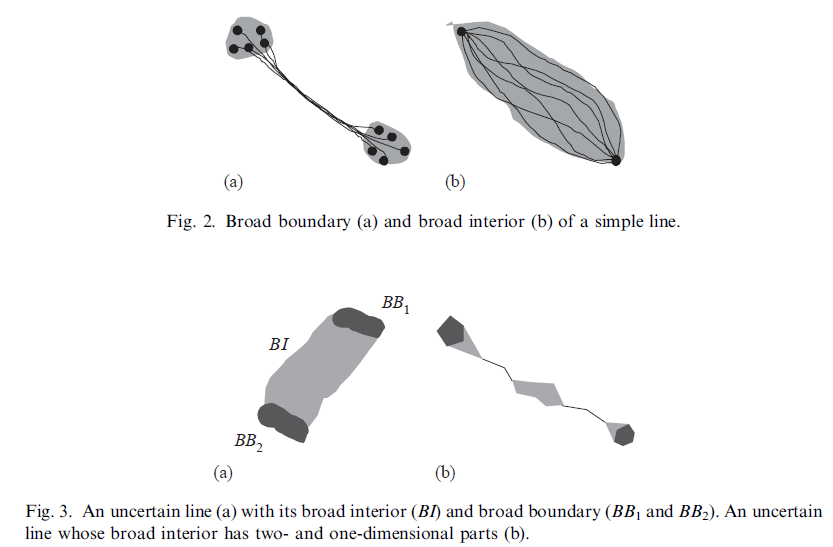
\includegraphics[height=0.7\textheight]{./Images/clem.png}
				%
				\caption{Proposition de modélisation de lignes imprécises, Clementini (2005)}
			\end{figure}
		}
	\end{overprint}	
\end{frame}


\begin{frame}{Schneider (1996)}
	 \begin{alertblock}{Proposition}
	 	\begin{itemize}
			\item Définir deux frontières par région à partir d'un semi discret (contrairement au paradigme des ensembles de points implicitement utilisé par les autres modèles)
		\end{itemize}
	\end{alertblock}
	\begin{exampleblock}{Limites}
		\begin{itemize}
		\item Celles du modèle \emph{egg-yolk}
		\item Approximation dans la modélisation
	\end{itemize}
	\end{exampleblock}
\end{frame}

\begin{frame}{Bejaoui (2009)}
	\begin{overprint}
		\only<1,3>{	
			\begin{alertblock}{Proposition}
				Étendre le modèle \emph{egg-yolk} en y ajoutant :
				\begin{itemize}
					\item La prise en compte d'objets partiellement imprécis
					\item La possibilité de modéliser des points et des lignes
				\end{itemize}  
			\end{alertblock}
		}
		\only<3>{
			\begin{exampleblock}{Limites}
				\begin{itemize}
					\item Complexifie énormément le modèle \emph{egg-yolk}
					\item Appartenance discrète
				\end{itemize}		
			\end{exampleblock}
		}
		\only<2>{
			\begin{figure}
			\centering
			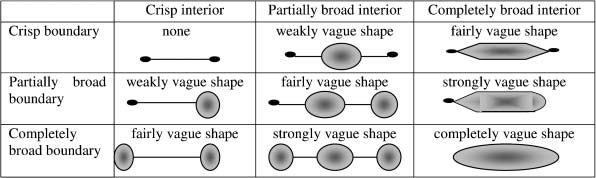
\includegraphics[width=\textwidth]{./Images/ligne_bejaoui.png}
			%
			\caption{Modélisation d'une ligne dans le modèle de Bejaoui}
		\end{figure}
		}
	\end{overprint}
\end{frame}


\subsection{Modèles basés sur la théorie des sous-ensembles flous}
\begin{frame}{Modèles flous}
	Le recours à la théorie des sous-ensembles flous offre plus de latitude dans la modélisation des géométrie imprécises 
		\begin{itemize}
			\item Théorie proposée par L. Zadeh en 1965
			\item Seule théorie mathématique modélisant l'imprécision
			\item Permet de modéliser des appartenances partielles
		\end{itemize}
\end{frame}

\begin{frame}{Modèles \og flous \fg}
	On peut distinguer deux catégories de méthodes de construction: 
	\begin{itemize}
		\item Définition en intention, \emph{i.e.} construction par règle 
		\item Définition en extension, \emph{i.e.} construction par sélection
	\end{itemize}
\end{frame}

\begin{frame}{Définition en intention, Schneider (1999)}
	 \begin{alertblock}{Proposition}
		\begin{itemize}
			\item les points sont définis comme un ensemble flou de coordonnées (x,y)
			\item Les lignes sont un ensemble spécifique de points flous
			\item les régions sont un ensemble spécifique de lignes floues
		\end{itemize}
	\end{alertblock}
	\begin{exampleblock}{Limites}
		\begin{itemize}
		\item Approche plus compliquée que les modèles \og exacts \fg
		\item Difficulté d'implémentation
	\end{itemize}
	\end{exampleblock}
\end{frame}

\begin{frame}{Définition en extension}
	\begin{overprint}
		\only<1,3>{
			 \begin{alertblock}{Proposition}
				\begin{itemize}
					\item Définir un maillage
					\item Définir les fonctions d'appartenance
					\item Calculer le degré d'appartenance pour chaque cellule
				\end{itemize}
			\end{alertblock}
	}
	\only<3>{
		\begin{exampleblock}{Limites}
			\begin{itemize}
				\item Impose une discrétisation de l'espace (raster)
			\end{itemize}
		\end{exampleblock}
	}
	\only<2>{
		\begin{figure}
			\centering
			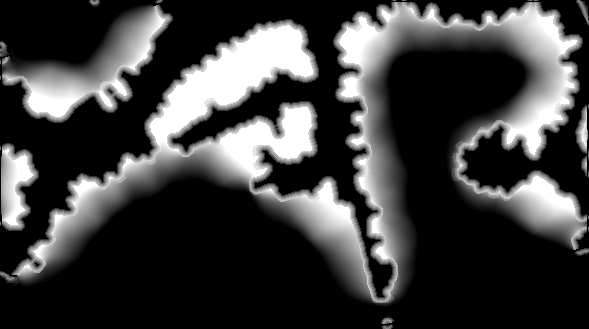
\includegraphics[width=\textwidth]{./Images/vanegass.png}
			%
			\caption{\emph{A fuzzy definition of the spatial relation “surround”,} Vanegass \emph{et al.} (2011)}
		\end{figure}
		}
	\end{overprint}
\end{frame}

\subsection{Modèles basés sur la théorie des probabilités}
\begin{frame}{Modèles probabilistes}
	\begin{itemize}
		\item Modélisation d'objets spatiaux imprécis à l'aide de la théorie des probabilités
		\item Modélisation de l'incertitude, mais non de l'imprécision
		\item Peu de modèles proposés
	\end{itemize}
\end{frame}

\begin{frame}{Tøssebro et Nygård (2002, 2008)}
	\begin{overprint}
		\only<1,3>{	
			\begin{alertblock}{Proposition}
				\begin{itemize}
					\item Les différents types sont modélisés à l'aide d'une région, d'un objet spatial net représentant le noyau et d'une fonction de probabilité
					\item Le modèle permet la modélisation de l'incertitude positionnelle, morphologique  et le doute sur l’existence de l’objet
				\end{itemize}  
			\end{alertblock}
		}
		\only<3>{
			\begin{exampleblock}{Limites}
				\begin{itemize}
					\item Ne modélise que l'incertitude
				\end{itemize}		
			\end{exampleblock}
		}
		\only<2>{
			\begin{figure}
			\centering
			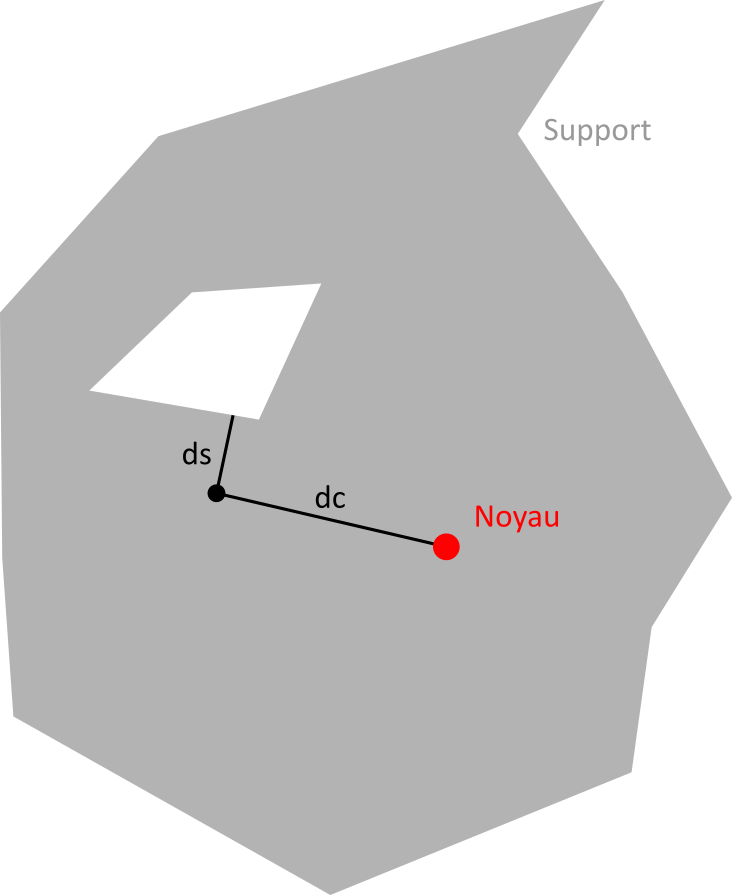
\includegraphics[height=0.6\textheight]{./Images/pointIncert.png}
			%
			\caption{Modélisation d'un point avec le modèle de Tøssebro et Nygård}
		\end{figure}
		}
	\end{overprint}
\end{frame}

\section{Cas d’applications}

\begin{frame}{Délimitation d'aires à partir de concepts vagues}
  	\begin{figure}
		\centering
		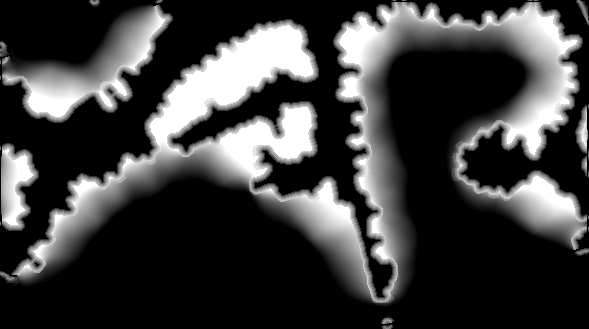
\includegraphics[width=\textwidth]{./Images/vanegass.png}
		%
		\caption{\emph{A fuzzy definition of the spatial relation “surround”,} Vanegass \emph{et al.} (2011)}
	\end{figure}
\end{frame}

\begin{frame}{Délimitation d'aires à partir de concepts vagues}
  	\begin{figure}
		\centering
		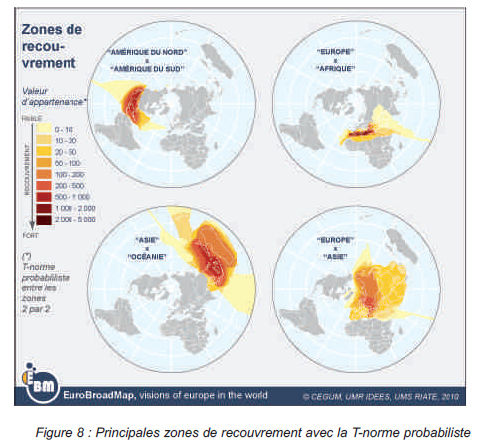
\includegraphics[height=0.7\textheight]{./Images/DidelonImp.png}
		%
		\caption{\emph{Un monde d'interstices,} Didelon \emph{et al.} (2009)}
	\end{figure}
\end{frame}

\begin{frame}{Calcul d'indices \og intuitifs \fg}
  	\begin{figure}
		\centering
		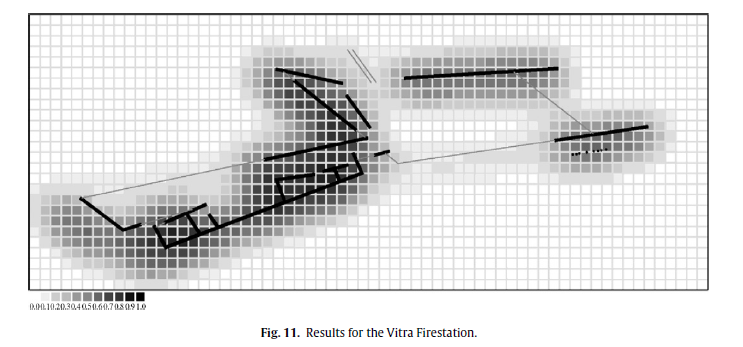
\includegraphics[width=\textwidth]{./Images/AddMod2.png}
		%
		\caption{\emph{Using fuzzy inference system for architectural space analysis,} Arabacioglu (2010)}
	\end{figure}
\end{frame}

\begin{frame}{Sélection floue}
  	\begin{figure}
		\centering
		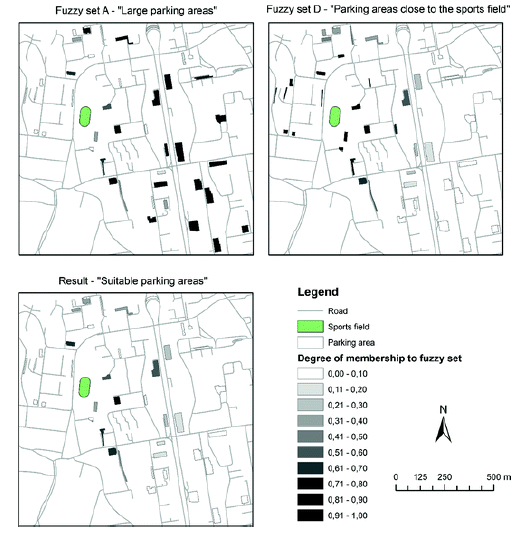
\includegraphics[height=0.7\textheight]{./Images/DurMod.png}
		%
		\caption{\emph{Fuzzy Spatio-Temporal Querying the PostgreSQL/PostGIS Database for Multiple Criteria Decision Making,}  Ďuračiová et Chalachanová  (2017)}
	\end{figure}
\end{frame}

\end{document}
